\documentclass[aspectratio=169, handout]{beamer}

%\usepackage[table]{xcolor}
\mode<presentation> {
\setbeamercovered{transparent}
  \usetheme{Boadilla}

\renewcommand{\familydefault}{cmss}
\usepackage{bm}
\usepackage{listings}
\useinnertheme{rectangles}
}
\usepackage{amsmath}
\usepackage{bbold}
\usepackage{tcolorbox}
\setbeamercolor{normal text}{fg=black}
\setbeamercolor{structure}{fg= blue}
\definecolor{trial}{cmyk}{1,0,0, 0}
\definecolor{trial2}{cmyk}{0.00,0,1, 0}
\definecolor{darkgreen}{rgb}{0,.4, 0.1}
\definecolor{darkpurple}{rgb}{0.4, 0, 0.6}
\usepackage{array}
\beamertemplatesolidbackgroundcolor{white}  \setbeamercolor{alerted
text}{fg=darkpurple}
\setbeamertemplate{caption}[numbered]\newcounter{mylastframe}

\font\domino=domino
\def\die#1{{\domino#1}}
\usepackage{tikz}
\usetikzlibrary{arrows}
\usepackage{colortbl}

\renewcommand{\familydefault}{cmss}

\usepackage{tikz}
\usepackage{lipsum}
\usepackage{booktabs}

\lstset{%
  language=R,
  basicstyle=\ttfamily\small,
  keywordstyle=\color{blue},
  commentstyle=\color{darkgreen},
  stringstyle=\color{darkpurple},
  showstringspaces=false,
  breaklines=true,
  frame=single,
  backgroundcolor=\color{gray!10}
}

 \newenvironment{changemargin}[3]{%
 \begin{list}{}{%
 \setlength{\topsep}{0pt}%
 \setlength{\leftmargin}{#1}%
 \setlength{\rightmargin}{#2}%
 \setlength{\topmargin}{#3}%
 \setlength{\listparindent}{\parindent}%
 \setlength{\itemindent}{\parindent}%
 \setlength{\parsep}{\parskip}%
 }%
\item[]}{\end{list}}
\usetikzlibrary{arrows}
\usetikzlibrary{arrows.meta, positioning}
\usepackage{pgfplots}
\pgfplotsset{compat=1.17}
\usecolortheme{lily}

\newtheorem{com}{Comment}
\newtheorem{lem} {Lemma}
\newtheorem{prop}{Proposition}
\newtheorem{condition}{Condition}
\newtheorem{thm}{Theorem}
\newtheorem{defn}{Definition}
\newtheorem{cor}{Corollary}
\newtheorem{obs}{Observation}
 \numberwithin{equation}{section}

\makeatletter
\def\beamerorig@set@color{%
  \pdfliteral{\current@color}%
  \aftergroup\reset@color
}
\def\beamerorig@reset@color{\pdfliteral{\current@color}}
\makeatother
\setbeamertemplate{navigation symbols}{}

\useoutertheme{miniframes}
\title[PLSC 30700]{Linear Models Lecture 16: GMM Inference and Going Beyond ATE}

\author{Robert Gulotty}
\institute[Chicago]{University of Chicago}
\vspace{0.3in}


\begin{document}

%========================================================
% SECTION 1: RECAP AND TESTING
%========================================================
\section{Recap and Testing}

%--- Slide 1: Title ---
\begin{frame}
\titlepage
\end{frame}

%--- Slide 2: Recap ---
\begin{frame}{Recap: The GMM Framework}

From Lecture 15:

\medskip
\textbf{The GMM estimator} minimizes the weighted quadratic form:
$$\hat\beta_{\text{gmm}} = \arg\min_\beta\; n\,\bar{g}_n(\beta)' W\, \bar{g}_n(\beta)$$

\medskip
\textbf{Key results:}
\begin{itemize}
\item $W = (Z'Z)^{-1}$ gives 2SLS (Thm 13.2)
\item Sandwich variance: $V_\beta = (Q'WQ)^{-1}(Q'W\Omega WQ)(Q'WQ)^{-1}$ (Thm 13.3)
\item Efficient GMM: $W = \Omega^{-1}$, $V_\beta = (Q'\Omega^{-1}Q)^{-1}$ (Thm 13.4)
\item 2SLS efficient only under homoskedasticity (Thm 13.6)
\item Two-step and iterated GMM are asymptotically efficient (Thm 13.7)
\end{itemize}

\medskip
\textbf{Today:} What can we \textit{test} with GMM? And how does GMM let us go \textit{beyond} average treatment effects?

\end{frame}

%--- Slide 3: J-Test Intuition ---
\begin{frame}{The Overidentification Test: Intuition}

When $\ell > k$, the model imposes \textbf{testable restrictions}.

\medskip
\textbf{Under correct specification:}
$$\mathbb{E}[g_i(\beta)] = 0 \quad\Rightarrow\quad \bar{g}_n(\hat\beta) \approx 0$$

Even at the minimizer, $\bar{g}_n(\hat\beta) \neq 0$ in finite samples. But it should be \textit{close} to zero.

\medskip
\textbf{Test logic:}
\begin{itemize}
\item \textbf{Small} $J(\hat\beta)$: Moment conditions are approximately satisfied $\Rightarrow$ model OK
\item \textbf{Large} $J(\hat\beta)$: Cannot simultaneously satisfy all moments $\Rightarrow$ \alert{misspecification}
\end{itemize}

\medskip
The criterion value $J = J(\hat\beta_{\text{gmm}})$ is a natural test statistic for:
$$H_0: \mathbb{E}[Ze] = 0 \qquad\text{vs.}\qquad H_1: \mathbb{E}[Ze] \neq 0$$

\end{frame}

%--- Slide 4: Hansen's J-Test (Thm 13.14) ---
\begin{frame}{Hansen's J-Test (Hansen Thm.~13.14)}

\begin{thm}[13.14: Overidentification Test]
Under $H_0: \mathbb{E}[Ze] = 0$ and using an efficient weight matrix estimator,
$$J = J(\hat\beta_{\text{gmm}}) = n\,\bar{g}_n(\hat\beta)'\hat\Omega^{-1}\bar{g}_n(\hat\beta) \xrightarrow{d} \chi^2_{\ell - k}$$

Reject $H_0$ if $J > \chi^2_{\ell-k,1-\alpha}$.
\end{thm}

\medskip
\textbf{Degrees of freedom} $= \ell - k =$ number of overidentifying restrictions.

\medskip
\textbf{Requirements:}
\begin{itemize}
\item Must use an \textit{efficient} weight matrix ($\hat W = \hat\Omega^{-1}$)
\item Generalizes the Sargan test (which assumed homoskedasticity)
\item When $\ell = k$ (just identified): $J = 0$ always --- \alert{no test possible}
\end{itemize}

\end{frame}

%--- Slide 5: J-Test Strengths and Limitations ---
\begin{frame}{J-Test: Strengths and Limitations}

\textbf{Strengths:}
\begin{itemize}
\item Automatic byproduct of efficient GMM estimation
\item General: works under heteroskedasticity, no distributional assumptions
\item Natural diagnostic: ``always report the J statistic'' (Hansen, Ch.~13)
\end{itemize}

\medskip
\textbf{Limitations:}
\begin{itemize}
\item \alert{No power if all instruments are invalid in the same direction} --- moments are all ``wrong'' together, J-test cannot detect this
\item Requires $\ell > k$ (overidentification)
\item Requires efficient weight matrix for $\chi^2$ distribution
\item Rejection tells you \textit{something} is wrong, but not \textit{what}
\end{itemize}

\smallskip
\alert{Good practice:} Use subset overidentification tests (Thm 13.15) to investigate \textit{which} instruments may be invalid.

\end{frame}

%--- Slide 6: J-Test for Missing Data ---
\begin{frame}[fragile]{J-Test for Missing Data}

From the Abrevaya \& Donald application (Lecture 15):

\begin{lstlisting}
# Run the specification test
specTest(gmm_men)

# Hansen's J-test
# Test E(g) = 0:
# Statistics  df  p-value
# J-test      ?   2    ?
\end{lstlisting}

\smallskip
\textbf{Interpretation} ($\ell - k = 7 - 5 = 2$ degrees of freedom):
\begin{itemize}
\item The test assesses whether the linear projection restriction holds for both missing and complete data subpopulations
\item \textbf{Fail to reject:} The restriction that $x = z'\gamma + \xi$ is the same for observed and missing cases is supported
\item \textbf{Reject:} Missingness may depend on unobservables, violating Assumption 1
\end{itemize}

\end{frame}

%========================================================
% SECTION 2: HYPOTHESIS TESTING
%========================================================
\section{Hypothesis Testing}

%--- Slide 7: The Wald Test (Thm 13.8) ---
\begin{frame}{The Wald Test (Hansen Thm.~13.8)}

Test $H_0: \theta = \theta_0$ where $\theta = r(\beta)$ for a known function $r: \mathbb{R}^k \to \mathbb{R}^q$.

\medskip
\begin{thm}[13.8: Wald Test]
Under $H_0$, as $n \to \infty$:
$$W = n(\hat\theta - \theta_0)'\hat V_\theta^{-1}(\hat\theta - \theta_0) \xrightarrow{d} \chi^2_q$$
where $\hat V_\theta = \hat R'\hat V_\beta \hat R$ and $\hat R = \frac{\partial}{\partial \beta}r(\hat\beta_{\text{gmm}})'$.
\end{thm}

\smallskip
\textbf{Special case:} Testing $\beta_j = 0$: $W = \hat\beta_j^2 / \widehat{\text{Var}}(\hat\beta_j) = t_j^2 \xrightarrow{d} \chi^2_1$

\medskip
\textbf{Familiar:} This is exactly the $t$-test (squared) we have been using throughout the course, now justified by GMM asymptotics.

\end{frame}

%--- Slide 8: The Distance Test (Thm 13.12) ---
\begin{frame}{The Distance Test (Hansen Thm.~13.12)}

An alternative to the Wald test, based on comparing criterion functions.

\smallskip
\textbf{Idea:} Estimate unrestricted ($\hat J$) and restricted ($\tilde J$, subject to $r(\beta)=\theta_0$) models by efficient GMM.

\begin{thm}[13.12: Distance Test]
Under $H_0$ and using efficient GMM, as $n \to \infty$:
$$D = \tilde J - \hat J \xrightarrow{d} \chi^2_q$$
\end{thm}

\smallskip
\textbf{Key advantages over Wald:}
\begin{itemize}\itemsep=1pt
\item \alert{Invariant to reparameterization}---the Wald statistic is not
\item Analogous to the likelihood ratio test (criterion-based)
\item Thm 13.13: If $\tilde\Omega = \hat\Omega$, then $D \geq 0$; for linear $r$, $D = W$
\end{itemize}

\end{frame}

%--- Slide 9: Three Tests Compared ---
\begin{frame}{Three Tests Compared}

\begin{table}[h]
\centering
\small
\begin{tabular}{p{2.8cm}p{3.5cm}p{3cm}p{3.5cm}}
\toprule
& \textbf{Wald Test} & \textbf{Distance Test} & \textbf{J-Test} \\
\midrule
\textbf{Tests} & Parameter restrictions $r(\beta) = \theta_0$ & Parameter restrictions $r(\beta) = \theta_0$ & Model specification $\mathbb{E}[g_i(\beta)] = 0$ \\[4pt]
\textbf{Requires} & Unrestricted estimate only & Both restricted and unrestricted & Efficient weight matrix \\[4pt]
\textbf{Distribution} & $\chi^2_q$ & $\chi^2_q$ & $\chi^2_{\ell - k}$ \\[4pt]
\textbf{Invariant?} & \alert{No} & Yes & N/A \\[4pt]
\textbf{Analogy} & $t$-test / $F$-test & Likelihood ratio & Sargan test \\
\bottomrule
\end{tabular}
\end{table}

\smallskip
\begin{tcolorbox}[colback=blue!5, colframe=blue!50]
\textbf{Recommendation:} Distance test for nonlinear hypotheses (invariant). Wald test for linear hypotheses (simpler, equivalent). Always report the J-test.
\end{tcolorbox}

\end{frame}

%--- Slide 10: Subset Overidentification (Thm 13.15) ---
\begin{frame}{Subset Overidentification Tests (Hansen Thm.~13.15)}

\textbf{Question:} Are \textit{specific} instruments valid?

\medskip
Partition $Z = (Z_a, Z_b)$ where:
\begin{itemize}
\item $Z_a$ ($\ell_a$ instruments): believed to be valid ($\mathbb{E}[Z_a e] = 0$)
\item $Z_b$ ($\ell_b$ instruments): questionable ($\mathbb{E}[Z_b e] \stackrel{?}{=} 0$)
\end{itemize}
Require $\ell_a > k$ so $Z_a$ alone identifies the model.

\smallskip
\begin{thm}[13.15: Subset Overidentification Test]
Let $\tilde J$ use only $Z_a$ and $\hat J$ use all $Z = (Z_a, Z_b)$. Then:
$$C = \hat J - \tilde J \xrightarrow{d} \chi^2_{\ell_b}$$
under $H_0: \mathbb{E}[Z_b e] = 0$.
\end{thm}

\medskip
\textbf{Special case:} If $Z_a$ is just-identified ($\ell_a = k$), then $\tilde J = 0$ and $C = \hat J$ is the standard J-test.

\end{frame}

%--- Slide 11: Endogeneity Test via GMM (Thm 13.16) ---
\begin{frame}{Endogeneity Test via GMM (Hansen Thm.~13.16)}

\textbf{Question:} Is $Y_2$ endogenous, i.e., is $\mathbb{E}[Y_2 e] \neq 0$?

\smallskip
Model: $Y = Z_1'\beta_1 + Y_2'\beta_2 + e$, \; instruments $(Z_1, Z_2)$ with $\mathbb{E}[Z_1 e]=\mathbb{E}[Z_2 e]=0$.

\smallskip
\textbf{Key insight:} If $Y_2$ is exogenous ($H_0$), then $Y_2$ is a \alert{valid instrument for itself}. So we can expand the instrument set from $(Z_1, Z_2)$ to $(Z_1, Z_2, Y_2)$.

\smallskip
\begin{thm}[13.16: Endogeneity Test]
\begin{enumerate}\itemsep=1pt
\item Estimate efficient GMM with instruments $(Z_1, Z_2)$. Let $\bar J$ be the criterion.
\item Estimate efficient GMM with instruments $(Z_1, Z_2, Y_2)$. Let $\hat J$ be the criterion.
\end{enumerate}
Under $H_0: \mathbb{E}[Y_2 e] = 0$, \; $C = \hat J - \bar J \xrightarrow{d} \chi^2_{k_2}$.
\end{thm}

\smallskip
This is a \textbf{subset overidentification test} where the ``questionable instruments'' are $Y_2$ itself. It \textbf{generalizes} Durbin-Wu-Hausman: DWH requires homoskedasticity; this GMM version does not.

\end{frame}

%--- Slide 12: GMM Subsumes All Prior Tests ---
\begin{frame}{GMM Subsumes All Prior Tests}

\begin{table}[h]
\centering
\small
\begin{tabular}{lll}
\toprule
\textbf{Earlier Course Test} & \textbf{GMM Version} & \textbf{Theorem} \\
\midrule
$t$-test for $\beta_j = 0$ & Wald test ($q = 1$) & 13.8 \\[3pt]
$F$-test for $R\beta = c$ & Wald test ($q > 1$) & 13.8 \\[3pt]
Hausman (OLS vs IV) & Endogeneity test & 13.16 \\[3pt]
Durbin-Wu-Hausman & Endogeneity test & 13.16 \\[3pt]
Sargan overid test & J-test & 13.14 \\[3pt]
White's heteroskedasticity test & Special case of J-test & --- \\[3pt]
Likelihood ratio test & Distance test & 13.12 \\
\bottomrule
\end{tabular}
\end{table}

\smallskip
\alert{Meta-lesson \#3 (General):} GMM provides a \textit{unified} framework for both estimation and inference. Every test we have seen is a special case of a GMM test---often under weaker assumptions.

\end{frame}

%========================================================
% SECTION 3: PROPAGANDA APPLICATION
%========================================================
\section{Application: Propaganda}

%--- Slide 13: When ATE Is Not Enough ---
\begin{frame}{When ATE Is Not Enough}

Recall from Lecture 14:
\begin{itemize}
\item \textbf{LATE} = effect for \textit{compliers} only --- those induced to change treatment by the instrument
\item Different instruments $\Rightarrow$ different complier groups $\Rightarrow$ \alert{different LATEs}
\end{itemize}

\medskip
\textbf{Key questions that LATE cannot answer:}
\begin{enumerate}
\item What is the effect for \textit{always-takers}? For \textit{never-takers}?
\item Does the treatment effect \textit{change sign} across subpopulations?
\item What would happen under a \textit{different policy} (different compliance margin)?
\end{enumerate}

\medskip
\begin{tcolorbox}[colback=blue!5, colframe=blue!50]
The \textbf{Marginal Treatment Effect} $\Delta^{MTE}(u_D)$ traces out treatment effects across the \textit{entire} resistance-to-treatment distribution. Estimating MTE requires GMM.
\end{tcolorbox}

\end{frame}

%--- Slide 14: West German TV in East Germany ---
\begin{frame}{West German TV in East Germany}

\textbf{Kern \& Hainmueller (2009):} Effect of Western media on support for the East German regime.

\medskip
\textbf{Setting:}
\begin{itemize}
\item Cold War East Germany (GDR), pre-1989
\item West German TV broadcast entertainment, news, and consumer culture
\item The regime feared Western media as subversive
\item Most East Germans could receive West German TV signals
\end{itemize}

\medskip
\textbf{Research question:} Did exposure to West German TV \textit{undermine} support for the Communist regime?

\medskip
\textbf{Outcome:} Support for the regime (survey data)

\textbf{Treatment:} Regular viewing of West German TV

\textbf{Challenge:} Viewers self-select into watching --- \alert{endogenous}

\end{frame}

%--- Slide 15: The Instrument: Geographic Signal Access ---
\begin{frame}{The Instrument: Geographic Signal Access}

\begin{center}
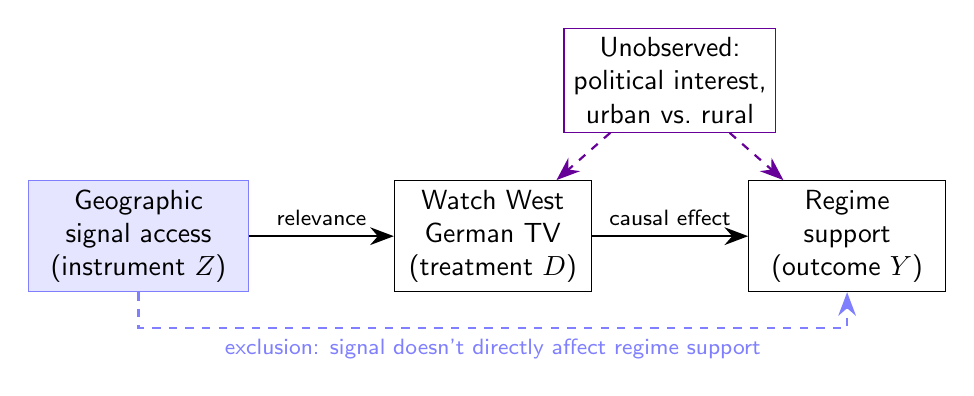
\begin{tikzpicture}[scale=0.9,
  box/.style={rectangle, draw, minimum height=1cm, minimum width=2.5cm, align=center},
  inst/.style={rectangle, draw=blue!50, fill=blue!10, minimum height=1cm, minimum width=2.8cm, align=center},
  arrow/.style={-{Stealth[length=3mm]}, thick}
]

\node[inst] (Z) at (0, 0) {Geographic\\signal access\\(instrument $Z$)};
\node[box] (D) at (5, 0) {Watch West\\German TV\\(treatment $D$)};
\node[box] (Y) at (10, 0) {Regime\\support\\(outcome $Y$)};
\node[box, draw=darkpurple, fill=white] (U) at (7.5, 2.2) {Unobserved:\\political interest,\\urban vs.\ rural};

\draw[arrow] (Z) -- (D) node[midway, above] {\footnotesize relevance};
\draw[arrow] (D) -- (Y) node[midway, above] {\footnotesize causal effect};
\draw[arrow, dashed, darkpurple] (U) -- (D);
\draw[arrow, dashed, darkpurple] (U) -- (Y);
\draw[arrow, dashed, blue!50] (Z) -- ++(0, -1.3) -| (Y) node[pos=0.25, below, font=\footnotesize] {exclusion: signal doesn't directly affect regime support};

\end{tikzpicture}
\end{center}

\medskip
\textbf{Key:} Due to topography and transmitter locations, some areas of East Germany could not receive West German TV --- notably the \textbf{Dresden} region (``Valley of the Clueless'').

\medskip
Geographic signal access is plausibly exogenous: determined by physics, not politics.

\end{frame}

%--- Slide 16: Conventional IV Results ---
\begin{frame}{Conventional IV Results}

\textbf{Standard IV/2SLS estimate:}

$$\widehat{LATE} \approx -0.12$$

\medskip
\textbf{Interpretation:} Among \textit{compliers} (those induced to watch by having signal access), watching West German TV reduces regime support by 0.12 standard deviations.

\medskip
\textbf{But who are the compliers?}
\begin{itemize}
\item People who watch West German TV \textit{only when they have signal access}
\item Not the most politically interested (they would find other sources --- always-takers)
\item Not the most regime-loyal (they would not watch even with access --- never-takers)
\item Compliers are a potentially \alert{narrow and unrepresentative} group
\end{itemize}

\medskip
\textbf{Question:} What about the effects for always-takers and never-takers?

\end{frame}

%--- Slide 17: MTE Results: Treatment Effect Heterogeneity ---
\begin{frame}{MTE Results: Treatment Effect Heterogeneity}

\textbf{Using the MTE framework} (extending Kern \& Hainmueller with MTE methods):

\medskip
\begin{table}[h]
\centering
\begin{tabular}{lcc}
\toprule
\textbf{Group} & \textbf{Treatment Effect} & \textbf{Interpretation} \\
\midrule
Always-takers & $-0.104$ & Western TV \textit{reduces} support \\
 & & (politically interested viewers) \\[6pt]
Compliers (LATE) & $\approx -0.12$ & Moderate effect \\[6pt]
Never-takers & $+0.189$ & Western TV \alert{\textit{increases}} support! \\
 & & (contrast effect / reactance) \\
\bottomrule
\end{tabular}
\end{table}

\smallskip
\alert{Sign reversal:} The treatment effect is \textit{negative} for willing viewers but \textit{positive} for resistant viewers! Western consumer culture made regime-loyal individuals \textit{more} supportive (reactance), while curious viewers became \textit{less} supportive (information effect).

\end{frame}

%--- Slide 18: Visualizing the MTE Curve ---
\begin{frame}{Visualizing the MTE Curve}

\begin{center}
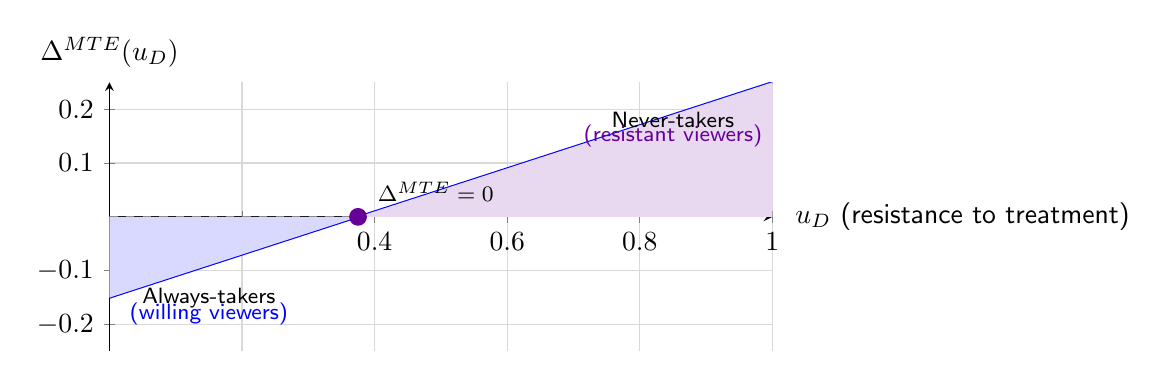
\begin{tikzpicture}
\begin{axis}[
  width=10cm, height=5cm,
  xlabel={$u_D$ (resistance to treatment)},
  ylabel={$\Delta^{MTE}(u_D)$},
  xmin=0, xmax=1, ymin=-0.25, ymax=0.25,
  xtick={0, 0.2, 0.4, 0.6, 0.8, 1.0},
  ytick={-0.2, -0.1, 0, 0.1, 0.2},
  axis lines=middle,
  grid=major,
  grid style={gray!30},
  every axis x label/.style={at={(ticklabel* cs:1.02)}, anchor=west},
  every axis y label/.style={at={(ticklabel* cs:1.02)}, anchor=south},
]

% MTE curve: starts negative, crosses zero, becomes positive
\addplot[domain=0:1, samples=100, thick, blue] {-0.15 + 0.40*x};

% Zero line
\addplot[domain=0:1, dashed, gray] {0};

% Shaded regions
\addplot[fill=blue!15, draw=none, domain=0:0.375, samples=50] {-0.15 + 0.40*x} \closedcycle;
\addplot[fill=darkpurple!15, draw=none, domain=0.375:1, samples=50] {-0.15 + 0.40*x} \closedcycle;

% Labels
\node[font=\footnotesize] at (axis cs:0.15, -0.15) {Always-takers};
\node[font=\footnotesize] at (axis cs:0.15, -0.18) {\color{blue}(willing viewers)};
\node[font=\footnotesize] at (axis cs:0.85, 0.18) {Never-takers};
\node[font=\footnotesize] at (axis cs:0.85, 0.15) {\color{darkpurple}(resistant viewers)};

% Mark the zero crossing
\addplot[mark=*, mark size=3pt, darkpurple] coordinates {(0.375, 0)};
\node[font=\footnotesize, anchor=south west] at (axis cs:0.39, 0.01) {$\Delta^{MTE} = 0$};

\end{axis}
\end{tikzpicture}
\end{center}

\textbf{Low $u_D$:} Always-takers (willing viewers) --- effect is \textit{negative}.
\textbf{High $u_D$:} Never-takers (resistant viewers) --- effect is \textit{positive}.
The \textbf{LATE} is a weighted average over compliers, masking the heterogeneity.

\end{frame}

%--- Slide 19: Why MTE Requires GMM ---
\begin{frame}{Why MTE Requires GMM}

\textbf{MTE estimation involves:}

\begin{enumerate}
\item \textbf{Nonlinear moment conditions:} $E[Y | X, Z] = X'\beta + \int_0^{P(Z)} \Delta^{MTE}(u)\, du$. Parameters enter through the integral --- nonlinear in $\beta$.

\smallskip
\item \textbf{Overidentification:} Multiple instruments provide more moment conditions than parameters $\Rightarrow$ testable.

\smallskip
\item \textbf{Efficient weighting:} Different propensity score regions are estimated with different precision $\Rightarrow$ optimal weighting matters.

\smallskip
\item \textbf{J-test:} Tests whether the MTE specification (e.g., polynomial degree) is adequate.
\end{enumerate}

\smallskip
\alert{Without GMM, we could not estimate or test the MTE.}

\end{frame}

%--- Slide 20: Policy Implications ---
\begin{frame}{Policy Implications}

The \textbf{Policy-Relevant Treatment Effect} (PRTE) depends on which part of the MTE curve the policy targets:

$$PRTE = \int_0^1 \Delta^{MTE}(u_D) \cdot \omega^{PRTE}(u_D)\, du_D$$

where $\omega^{PRTE}$ depends on how the policy shifts the propensity score.

\smallskip
\textbf{For the propaganda example:}
\begin{itemize}\itemsep=1pt
\item Forcing everyone to watch (shifting never-takers) could \alert{backfire}: MTE is positive for high $u_D$
\item Facilitating access for willing viewers (low $u_D$) would reduce regime support
\item The PRTE sign/magnitude depends on the policy's compliance margin
\end{itemize}

\smallskip
\alert{Lesson:} Treatment effect heterogeneity means policy evaluation requires more than a single number. The MTE curve---estimated via GMM---provides the necessary detail.

\end{frame}

%--- Slide 21: Connection to ivmte ---
\begin{frame}[fragile]{Connection to ivmte}

Recall from Lecture 14: the \texttt{ivmte} package (Shea \& Torgovitsky) estimates MTE:

\begin{lstlisting}[basicstyle=\ttfamily\footnotesize]
library(ivmte)
result <- ivmte(
  data = df,
  outcome = "regime_support",
  treatment = "watch_western_tv",
  instrument = "signal_access",
  target = "ate",       # or "att", "prte"
  m0 = ~ u + I(u^2),   # MTE polynomial for control
  m1 = ~ u + I(u^2),   # MTE polynomial for treated
  propensity = D ~ signal_access
)
\end{lstlisting}

\smallskip
\textbf{Under the hood, \texttt{ivmte} performs:} nonlinear GMM estimation of MTE parameters, efficient weighting across moment conditions, and overidentification testing (J-test).

\end{frame}

%========================================================
% SECTION 4: COURSE INTEGRATION
%========================================================
\section{Course Integration}

%--- Slide 22: Restricted GMM (Hansen 13.15--16) ---
\begin{frame}{Restricted GMM (Hansen \S13.15--13.16)}

\textbf{Linear constraints:} $R'\beta = c$

\smallskip
$\hat\beta_{\text{cgmm}} = \hat\beta_{\text{gmm}} - (X'ZWZ'X)^{-1}R\!\left(R'(X'ZWZ'X)^{-1}R\right)^{-1}\!(R'\hat\beta_{\text{gmm}} - c)$

\smallskip
This is the GMM analog of restricted OLS / minimum distance.

\medskip
\textbf{Nonlinear constraints:} $r(\beta) = 0$ --- minimize $J(\beta)$ subject to constraint (numerical optimization).

\medskip
\begin{thm}[13.10--13.11]
The constrained efficient GMM estimator has asymptotic variance
$V_{\text{cgmm}} = V_\beta - V_\beta R(R'V_\beta R)^{-1}R'V_\beta$.
Constrained estimation is (weakly) more efficient than unconstrained --- if the constraints are true.
\end{thm}

\end{frame}

%--- Slide 23: Bootstrap for GMM (Hansen 13.26) ---
\begin{frame}{Bootstrap for GMM (Hansen \S13.26)}

Standard bootstrap for GMM: resample $(Y_i^*, X_i^*, Z_i^*)$ and re-estimate.

\medskip
\alert{Problem:} When overidentified, the bootstrap estimator does not satisfy the orthogonality condition $\Rightarrow$ no asymptotic refinement.

\medskip
\textbf{Solution: Recentered bootstrap} (Hall \& Horowitz, 1996)
$$\hat\beta_{\text{gmm}}^{**} = (X^{*\prime}Z^*W^*Z^{*\prime}X^*)^{-1}(X^{*\prime}Z^*W^*(Z^{*\prime}Y^* - Z'\hat e))$$
where $\hat e = Y - X\hat\beta_{\text{gmm}}$ from the \textit{original} sample. Subtracts original residuals' moment contribution to recenter around zero.

\medskip
\textbf{Practical advice:} Use bootstrap for confidence intervals (not SEs). Percentile-$t$ bootstrap provides best finite-sample coverage.

\end{frame}

%--- Slide 24: The Full GMM Testing Toolkit ---
\begin{frame}{The Full GMM Testing Toolkit}

\begin{table}[h]
\centering
\small
\begin{tabular}{p{3.5cm}lp{3.5cm}}
\toprule
\textbf{Test} & \textbf{Distribution} & \textbf{Purpose} \\
\midrule
J-test (Thm 13.14) & $\chi^2_{\ell-k}$ & Model specification \\[3pt]
Wald (Thm 13.8) & $\chi^2_q$ & Parameter restrictions \\[3pt]
Distance (Thm 13.12) & $\chi^2_q$ & Parameter restrictions (invariant) \\[3pt]
Subset overid (Thm 13.15) & $\chi^2_{\ell_b}$ & Validity of specific instruments \\[3pt]
Endogeneity (Thm 13.16) & $\chi^2_{k_2}$ & Exogeneity of regressors \\[3pt]
Constrained (Thm 13.10) & --- & Efficient estimation under $H_0$ \\[3pt]
Bootstrap & --- & Finite-sample inference \\
\bottomrule
\end{tabular}
\end{table}

\smallskip
\textbf{All tests are:} valid under heteroskedasticity, derived from the GMM criterion function, and applicable to both linear and nonlinear models.

\end{frame}

%--- Slide 25: Semiparametric Efficiency Bound ---
\begin{frame}{Semiparametric Efficiency Bound}

\textbf{Chamberlain (1987):} If all that is known is $\mathbb{E}[g_i(\beta)] = 0$, this is a \textbf{semiparametric} problem (the distribution of the data is unknown).

\medskip
Chamberlain showed that no semiparametric estimator can have asymptotic variance smaller than $(G'\Omega^{-1}G)^{-1}$ where $G = \mathbb{E}\!\left[\frac{\partial}{\partial \beta'}g_i(\beta)\right]$.

\medskip
\textbf{Efficient GMM achieves this bound:} $V_\beta = (Q'\Omega^{-1}Q)^{-1} = (G'\Omega^{-1}G)^{-1}$

\medskip
\begin{tcolorbox}[colback=blue!5, colframe=blue!50]
\textbf{This means:}
\begin{itemize}
\item No other estimator using only these moment conditions can do better
\item MLE \textit{can} do better --- but requires specifying the full distribution
\item GMM is the best you can do without distributional assumptions
\end{itemize}
\end{tcolorbox}

\end{frame}

%--- Slide 26: When to Use GMM vs. Other Methods ---
\begin{frame}{When to Use GMM vs.\ Other Methods}

\begin{table}[h]
\centering
\small
\begin{tabular}{p{1.5cm}p{3.8cm}p{3.8cm}p{2.8cm}}
\toprule
& \textbf{When to use} & \textbf{Advantages} & \textbf{Cost} \\
\midrule
\textbf{OLS/GLS} & $\mathbb{E}[Xe]\!=\!0$ (no endogeneity) & Simple, efficient under assumptions & Biased if endogenous \\[3pt]
\textbf{2SLS} & Endogeneity, homoskedastic & Simple, familiar & Inefficient under heterosked. \\[3pt]
\textbf{GMM} & Endogeneity, heteroskedastic & Efficient, flexible, testable & More complex \\[3pt]
\textbf{MLE} & Full distribution known & Most efficient (Cram\'er--Rao) & Misspecification bias \\
\bottomrule
\end{tabular}
\end{table}

\smallskip
\textbf{Decision rule:}
\begin{itemize}\itemsep=1pt
\item No endogeneity? $\Rightarrow$ OLS/GLS
\item Endogeneity + homoskedasticity + few instruments? $\Rightarrow$ 2SLS
\item Endogeneity + heteroskedasticity or many instruments? $\Rightarrow$ \textbf{GMM}
\item Full distributional knowledge? $\Rightarrow$ MLE
\end{itemize}

\end{frame}

%--- Slide 27: The Three Meta-Lessons Revisited ---
\begin{frame}{The Three Meta-Lessons Revisited}

\begin{enumerate}
\item \textbf{Semiparametric}
\begin{itemize}
\item Requires only moment conditions --- achieves Chamberlain bound
\item Missing data: no distributional assumptions on missingness
\item MTE: no parametric model for selection --- only moments from the propensity score
\end{itemize}

\smallskip
\item \textbf{Efficient}
\begin{itemize}
\item Optimal weighting $W = \Omega^{-1}$ minimizes variance
\item Missing data: GMM has lowest MSE across methods
\item Propaganda: efficient weighting across propensity score values
\end{itemize}

\smallskip
\item \textbf{General}
\begin{itemize}
\item Unified estimation: OLS, GLS, IV, 2SLS all as special cases
\item Unified testing: $t$, $F$, Hausman, Sargan all as special cases
\item Extends to nonlinear models, treatment effect heterogeneity, policy evaluation
\end{itemize}
\end{enumerate}

\end{frame}

%--- Slide 28: The Course in One Slide ---
\begin{frame}{The Course in One Slide}

\begin{center}
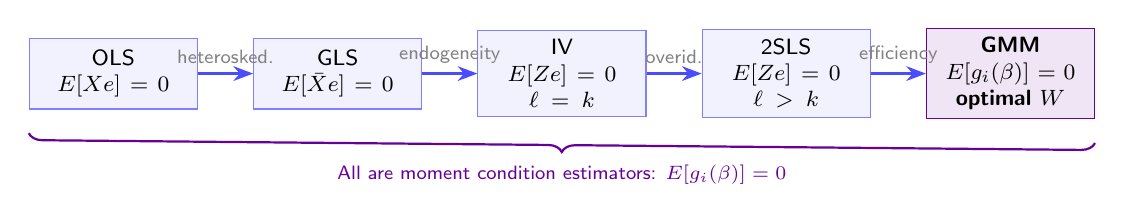
\begin{tikzpicture}[
  node distance=0.6cm and 0.7cm,
  box/.style={rectangle, draw=blue!50, fill=blue!5, text width=1.9cm, minimum height=0.9cm, align=center, font=\footnotesize},
  gmmbox/.style={rectangle, draw=darkpurple, fill=darkpurple!10, text width=1.9cm, minimum height=0.9cm, align=center, font=\footnotesize\bfseries},
  arrow/.style={-{Stealth[length=2.5mm]}, thick, blue!70},
  label/.style={font=\scriptsize, text=gray}
]

\node[box] (ols) {OLS\\$E[Xe]=0$};
\node[box, right=of ols] (gls) {GLS\\$E[\bar Xe]=0$};
\node[box, right=of gls] (iv) {IV\\$E[Ze]=0$\\$\ell = k$};
\node[box, right=of iv] (tsls) {2SLS\\$E[Ze]=0$\\$\ell > k$};
\node[gmmbox, right=of tsls] (gmm) {GMM\\$E[g_i(\beta)]=0$\\optimal $W$};

\draw[arrow] (ols) -- (gls) node[midway, above, label] {heterosked.};
\draw[arrow] (gls) -- (iv) node[midway, above, label] {endogeneity};
\draw[arrow] (iv) -- (tsls) node[midway, above, label] {overid.};
\draw[arrow] (tsls) -- (gmm) node[midway, above, label] {efficiency};

% Bottom: moment condition unification
\draw[decorate, decoration={brace, amplitude=5pt, mirror}, thick, darkpurple]
  ([yshift=-3mm]ols.south west) -- ([yshift=-3mm]gmm.south east)
  node[midway, below=6pt, font=\scriptsize, text=darkpurple] {All are moment condition estimators: $\mathbb{E}[g_i(\beta)] = 0$};

\end{tikzpicture}
\end{center}

\smallskip
\textbf{The progression:} Each step addresses a \textit{new problem} (heteroskedasticity, endogeneity, overidentification, efficiency). Each estimator is a \textit{special case} of the next. GMM is the \textit{most general}: it nests everything and achieves the semiparametric bound.

\end{frame}

%--- Slide 29: Looking Ahead: Panel Data ---
\begin{frame}{Looking Ahead: Panel Data}

\textbf{Next week: Panel data and fixed effects}

\medskip
Panel data (repeated observations on the same units) introduces new moment conditions:

\medskip
\textbf{Fixed effects as moments:}
$$\mathbb{E}[\tilde X_i \tilde e_i] = 0 \qquad\text{(within-group orthogonality)}$$
where $\tilde X_i = X_{it} - \bar X_i$ is the demeaned regressor.

\medskip
\textbf{Arellano-Bond (1991) GMM:}
\begin{itemize}
\item Dynamic panels: $Y_{it} = \rho Y_{it-1} + X_{it}'\beta + \alpha_i + e_{it}$
\item Lagged levels as instruments for first-differenced equation
\item Growing set of moment conditions: $\mathbb{E}[\Delta e_{it} \cdot Y_{is}] = 0$ for $s \leq t-2$
\item Naturally overidentified $\Rightarrow$ GMM with efficient weighting + J-test
\end{itemize}

\medskip
\alert{GMM is the workhorse estimator for dynamic panel data.}

\end{frame}

%--- Slide 30: Summary ---
\begin{frame}{Summary}

\textbf{Five takeaways from Lectures 15--16:}

\smallskip
\begin{enumerate}\itemsep=2pt
\item \textbf{GMM is a unified estimation framework} that nests OLS, GLS, IV, and 2SLS as special cases, requiring only moment conditions $\mathbb{E}[g_i(\beta)] = 0$.

\item \textbf{Efficient GMM} uses $W = \Omega^{-1}$ to achieve the semiparametric efficiency bound. Two-step and iterated GMM achieve this in practice.

\item \textbf{The J-test} provides a natural diagnostic for overidentified models. Always report it.

\item \textbf{GMM subsumes all prior tests:} Wald, Distance, subset overidentification, and endogeneity tests are all GMM tests---valid under heteroskedasticity.

\item \textbf{Going beyond ATE:} GMM enables estimation of the MTE curve, revealing treatment effect heterogeneity that LATE conceals.
\end{enumerate}

\end{frame}

\end{document}
